\documentclass[a4paper,spanish]{article}

\usepackage[utf8]{inputenc}
\usepackage[spanish, es-tabla]{babel}
\usepackage[T1]{fontenc}
\usepackage[margin={18mm, 26mm}]{geometry}
\usepackage[hidelinks]{hyperref}

\usepackage{graphicx}
\graphicspath{ {./assets/img/} }


\usepackage{fancyhdr}
\pagestyle{fancy}
\fancyhead{}
\fancyfoot{}
\fancyhead[C]{ \date{\today} $\bullet$ G.I.R. - Probabilidad y Estadística Matemática $\bullet$ Prácticas Externas}
\fancyfoot[RO,LE]{\thepage}
%----------------------------------------------------------------------------------------
%	TITLE SECTION
%----------------------------------------------------------------------------------------

%----------------------------------------------------------------------------------------

\begin{document}
	\begin{titlepage}
	\centering
    
\includegraphics[width=0.5\textwidth]{logo_uva}
    \par\vspace{0.5cm}
    {\scshape\large Grado en Estadística - Facultad de Ciencias \par}
		\vspace{1cm}
		{\scshape\LARGE G.I.R. - Probabilidad y Estadística Matemática\par}
		\vspace{1.5cm}
		{\Huge\bfseries Prácticas Externas\par}
		\vspace{2cm}
		{\large
		\textsc{Sergio García Prado\textsubscript}\\[2mm] % Your name
		\vspace{-5mm}
		}

		\vfill

	% Bottom of the page
		{\large \today\par}
	\end{titlepage}

	\thispagestyle{fancy} % All pages have headers and footers

%----------------------------------------------------------------------------------------
%	TABLE OF CONTENTS
%----------------------------------------------------------------------------------------

	\tableofcontents
	\newpage

%----------------------------------------------------------------------------------------
%	TEXT
%----------------------------------------------------------------------------------------



  \section{Datos Generales de la Práctica}


    \subsection{Datos personales del alumno}

      \begin{itemize}
        \item \emph{Nombre y apellidos:} Sergio García Prado
        \item \emph{Dirección:} La Paz, 7 3C
        \item \emph{Localidad:} Palencia 34002, España
        \item \emph{Teléfono:} +34 696 904 878
        \item \emph{Email:} sergio.garcia.prado@alumnos.uva.es
      \end{itemize}


    \subsection{Datos de la empresa}

      \begin{itemize}
        \item \emph{Nombre de la empresa:} Universidad de Valladolid (G.I.R. - Probabilidad y Estadística Matemática)
        \item \emph{Dirección:} Paseo Belén, 7
        \item \emph{Localidad:} Valladolid
        \item \emph{Teléfono:} +34 983 423 016
      \end{itemize}


    \subsection{Tutor en la Empresa}

      \begin{itemize}
        \item \emph{Nombre y apellidos:} Pedro Cesar Alvarez Esteban
        \item \emph{Cargo en la empresa:} Coordinador
        \item \emph{Email:} lagarcia@eio.uva.es
      \end{itemize}


    \subsection{Calendario y horario de las prácticas}

      \begin{itemize}
        \item \emph{Días semanales:} Lunes a Viernes
        \item \emph{Horario diario:} 4 horas
        \item \emph{Fecha de inicio:} 12/03/2018
        \item \emph{Fecha de fin:} 29/05/2018
        \item \emph{Total horas realizadas:} 150 horas
      \end{itemize}

	\newpage
  \section{Breve Descripción de la Empresa}

    \paragraph{}
    [TODO]

  \section{Memoria de Actividades}

    \paragraph{}
    [TODO]


  \section{Utilidad como complemento a la formación universitaria}

    \paragraph{}
    [TODO]


  \section{Utilidad para la futura inserción laboral}

    \paragraph{}
    [TODO]


  \section{Valoración personal y Sugerencias de mejora}

    \paragraph{}
    [TODO]

  \newpage
   \section{Declaración de Responsabilidad}

       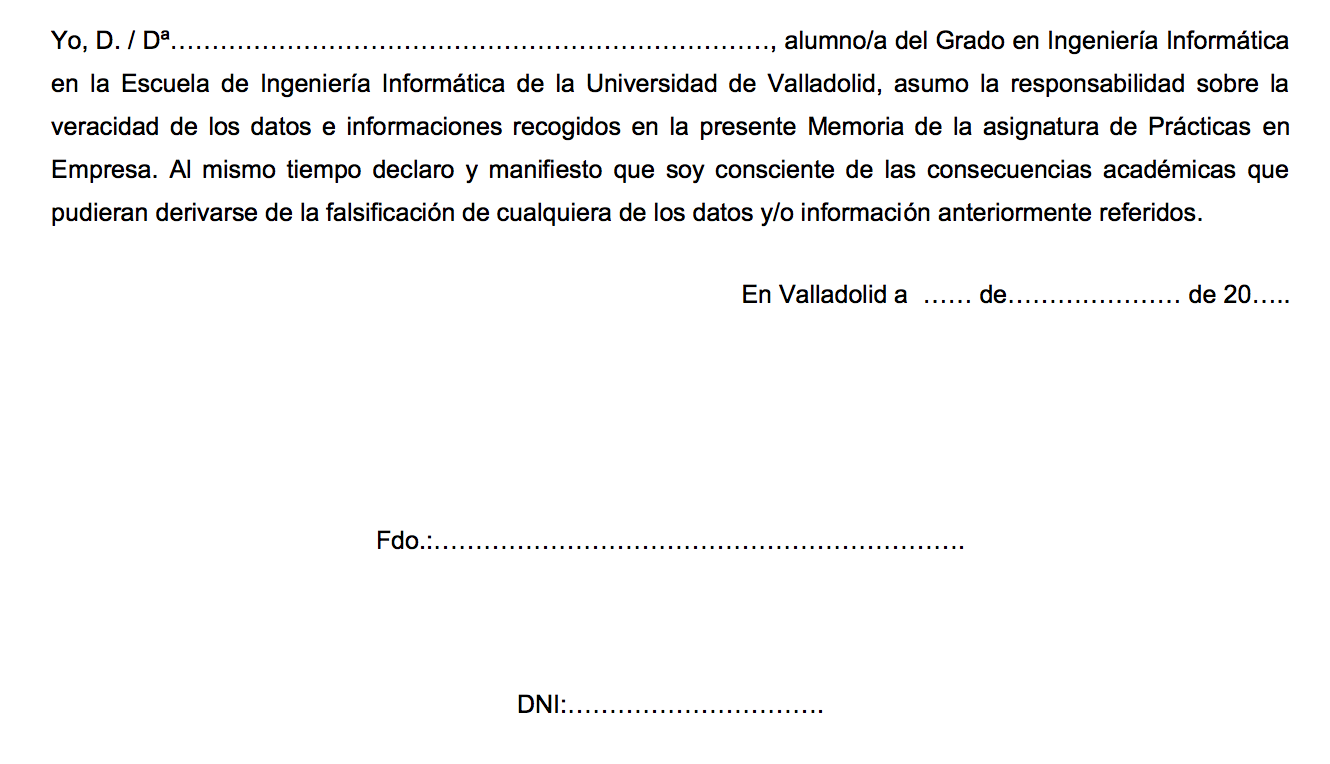
\includegraphics[width=\textwidth]{responsibility-declaration}


\end{document}
